%----------------------------------------
% Write your notes here
%----------------------------------------
\section{What is Hadoop?}
\begin{itemize}
	\item An abstraction for parallel data analysis
	\item consists of many subprojects
		\subitem - we will mostly focus on Map/Reduce
	\item deals with distributed data
	\item born out of open source web indexing, crawling, and searching software
	\item Map/Reduce revealed by Google in 2004
		\subitem - added to Hadoop, which is adopted by Yahoo! in 2006
\end{itemize}

\section{Why do we need Map/Reduce?}
\begin{itemize}
	\item There is still a lot of latency when dealing with a lot of data
	\item Read speed of commodity hard disk is about 1 TB/4hrs
	\item Using Hadoop, 1PB can be sorted in 16.5 hours! \href{bit.ly/petabytesort}{petabytesort}
\end{itemize}

\section{Map/Reduce} 
\begin{itemize}
	\item break into parts
	\item process in parallel
	\item combine results
\end{itemize} 

For example, if we wanted to count the number of occurences of each word in a book:
\begin{enumerate} 
	\item For every word on every page
	\item Map to (word, count) e.g. ("cat", 1) 
	\item Shuffle to collect all records with the same key (word)
		\subitem hash(val) = hashVal mod number of reducers
	\item Reduce results by adding count values for each word 
\end{enumerate}

To use Map/Reduce, you must specify the Map and Reduce steps

\section{Principles}
\begin{itemize}
	\item move code to data
	\item allow programs to scale transparently 
\end{itemize}

\section{Strengths of Map/Reduce}
\begin{itemize}
	\item batch, offline
	\item write-once read-many
	\item simple computations
	\item I/O bound by disk or network bandwith
\end{itemize}

\section{Weaknesses}
\begin{itemize}
	\item does not work well for high performance parallel computing applications
	\item low latency on random access
	\item not always the right solution
	\item difficult to find points of failure
\end{itemize} 

Before you use Map/Reduce, you should make sure it's the right tool for the job. 

\section{Beware the Curse!}
\begin{itemize}
	\item often there is an assumption that all machines in the Map/Reduce pipeline end up with approximately the same amount of work
	\item this is not always true
		\subitem - not the case when working with skewed data
		\subitem - can do clever shuffles to avoid this if there is prior knowledge of skewness in the data
\end{itemize}

\newpage

\section{Examples} 
Below are two different examples of MapReduce, taken from "Cracking the Coding Interview, 6th Ed." by G. McDowell. 
	\subsection{WordCount} 
	See above.
	\begin{figure}[]
		\begin{center} 
			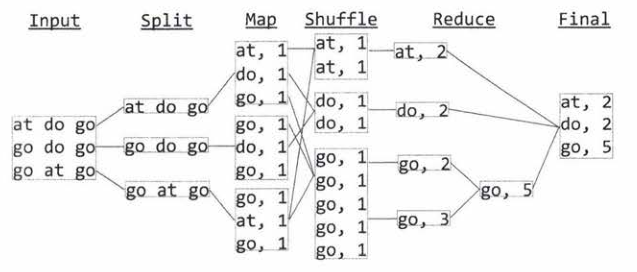
\includegraphics[width=0.5\textwidth]{figures/MR_1.png}
			\caption{In this example, we see a graphical representation of a word count program using Map/Reduce. The Map step emits tuples of (word, count). The Shuffle step brings all corresponding words together. The Reduce step adds the counts of all the corresponding words. In the final step we have a list of tuples, each with its own word and the count of that word in the original input.}
		\end{center}
	\end{figure}

	\subsection{Average Temperature}
	Say you are given a list of data in the form (City, Temperature, Date). You wish to find the average temperature for each city in a given year. How would you set up the Map and Reduce steps to perform this calculation? 
	
	\begin{itemize}
	\item \textbf{Map}: Given a data point, the Map step will emit a (Key, Value) tuple of the form (CityYear, [Temperature, N]). The "Key" will be a particular city and year. The "Value" will be a tuple of Temperature and N, where N indicates the associated temperature is the average of N data points. This will be important in the Reduce step. 
	\item \textbf{Reduce}: Given a list of emitted values, the Reduce step will take the weighted average of temperatures for each CityYear, where the weights will be N.
\end{itemize}	